\subsection{Securing network traffic}
The complex and distributed nature of the internet causes it to be inherently insecure. A network request may travel through switches located in a number of countries and operated by various actors, and the route might even change between requests as the network topology and load changes. As such, we have to assume that some link along the chain is listening to the traffic we send. In the context of web traffic, this lack of trust causes issues, as users want to be able to send potentially sensitive information with the knowledge that no external actor will be able to read or modify the data.

\subsubsection{Public key encryption}
To mitigate the risk of malicious parties being able to listen in on network communication, public-key encryption can be used.
Public key cryptography relies on a public-private key pair, where the public key is used to encrypt data and the private key is used to decrypt data.
A network actor can generate the key pair and send the public key to the other endpoint.
Since the public key can only be used to encrypt data, an attacker will not gain any valuable information if they are able to intercept the public key.
With the public key, the other endpoint can encrypt the data before sending it over a network.
Since the data can only be decrypted by the corresponding private key, a network attacker which successfully intercepts the communication is unable to read the original data \citep{hellman_overview_1978}.

Diffie-Hellman key exchange is one method to exchange keys for public key cryptography \citep{diffie_new_1976}  \citep{gillmor_negotiated_2016}.
\begin{enumerate}
    \item The Diffie-Hellman key exchange begins by two parties, Alice and Bob, agreeing on two publicly shared values, $p$, and $g$, where $p$ is a prime and $g$ is a primitive root modulo $p$.
    \item Alice chooses a secret integer $a$ and sends $A = g^a \mod p$ to Bob.
    \item Bob chooses a secret value $b$ and sends $B = g^b \mod p$ to Alice.
    \item Alice computes $s = B^a \mod p$
    \item Bob computes $s = A^b \mod p$
\end{enumerate}

Alice and Bob now share the secret $s$, since \[A^b \mod p = g^{ab} \mod p = g^{ba} \mod p = B^a \mod p\]
The secret share is considered secure, as finding $a$ and $b$ given $g^{ab} \mod p = g^{ba} \mod p$ takes a long time to compute with our current algorithms.

If Diffie-Hellman key exchange is used, an attacker can store large amounts of network traffic, with the hope of the secret key leaking in the future, thus allowing the attacker to decrypt all previous communication.
Additionally, in traditional public-key cryptography, the keys between two parties can stay constant for long amounts of time, allowing an attacker to decrypt all previous traffic at once if the secret is leaked in the future.
To protect against such attacks, short lived keys, commonly referred to as ephemeral keys, can be used, such as in the SAKE protocol \citep{jarecki_symmetric-key_2020}.
The SAKE protocol solves the issue of a future key leak being able to decrypt previous communication by continuously updating the secret key, making it impossible to derive an older secret key from a newer one.
Ensuring that an encryption scheme is resistant to keys being leaked at a later point is known as perfect forward secrecy.

\subsubsection{Transport Layer Security}
Today, the Transport Layer Security (TLS) protocol is used to prevent eavesdropping, tampering and forging messages in client-server communication. The latest version of the specification is TLS 1.3, which among other things removes insecure ciphers, allows for fewer round trips in the handshake and forces clients and servers to use ephemeral key exchange methods, ensuring perfect forward secrecy \citep{dowling_cryptographic_2015}. 

TLS provides a secure channel which provides authentication, confidentiality and integrity, even if an attacker has complete control of the network. The server is always authenticated, while the client can be optionally authenticated. The confidentiality of the transmitted data is ensured by encryption, only allowing the server and client to decrypt the contents. TLS 1.3 additionally ensures forward secrecy, effectively preventing attacks that store large amounts of encrypted data with the hope of decrypting it at a later point when keys are compromised. The lengths of the data and the identities of the client and server are however not hidden. Integrity is ensured by detecting any external modifications to the sent data.

The full TLS 1.3 handshake, described in figure \ref{tls}, functions as follows \citep{rescorla_transport_2018}:

\begin{figure}[b]
	\centering
	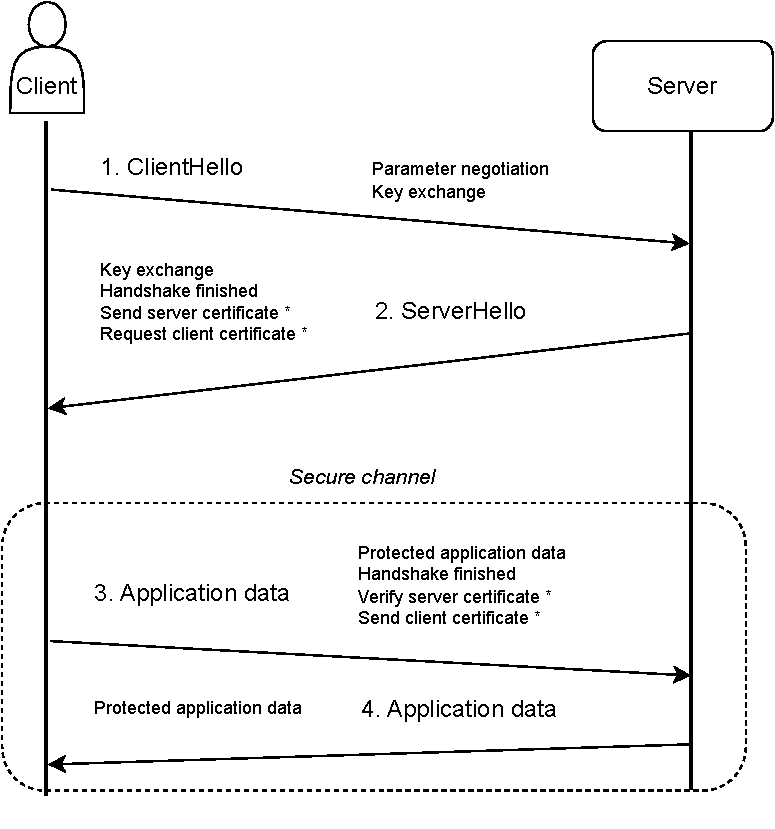
\includegraphics[height=120mm]{assets/tls_1.3_handshake.drawio.pdf}
	\caption{Full TLS 1.3 handshake. Optional content marked with *.}
	\label{tls}
\end{figure}

\begin{enumerate}
    \item The \textit{ClientHello} message is used for negotiating parameters and exchanging keys. The configurable parameters are TLS versions, groups, cipher suites and certificate authorities. The key exchange is initiated by sending the client's Diffie-Hellman key share. The client can request a server certificate, further ensuring that no impersonation attack can take place.
    \item \textit{ServerHello}: The server selects a cipher and TLS version based on the lists sent by the client and confirms that the handshake is finished. The server can suggest new parameters if it does not support any of the parameters sent by the client. The server also sends its own Diffie-Hellman key share and a server certificate, if one was requested. If client authentication is used, the server will request a client certificate. If a pre-shared key is used, the server can send application data in this message, allowing for data transfer without any additional round trips.
    \item A secure channel is established, allowing the client to send application data encrypted with the previously shared key. The client confirms that the handshake has been completed and sends a certificate if one was requested.
    \item The server can now use the secure channel to send encrypted application data.
\end{enumerate}
